\documentclass[class=jsarticle, crop=false, dvipdfmx, fleqn]{standalone}
%% preamble for Numerical-structure-analysis report

\input{/Users/User/Documents/Project/TeX/preamble/mypreamble}

%% titles
\title{先端データ解析論 レポート}
\author{37-196360 \quad 森田涼介}


%% setting for listings
\newtcbinputlisting[auto counter]{\reportlisting}[3][]{%
	listing file = {#3},
	listing options = {language=python, style=tcblatex, numbers=left, numberstyle=\tiny},
	listing only,
	breakable,
	toprule at break = 0mm,
	bottomrule at break = 0mm,
	left = 6mm,
	sharp corners,
	drop shadow,
	title = Listings \thetcbcounter : \texttt{#2},
	label = #1,
	}



%% title format
\usepackage{titlesec}
\titleformat{\section}{\LARGE}{宿題\thesection}{0zw}{}
\newcommand{\sectionbreak}{\clearpage}
\titleformat{\subsection}{\Large}{\Alph{subsection})}{0zw}{}

\begin{document}
\section{}


フィッシャー判別分析を実装する。

クラス内散布行列は,
\begin{equation}
    \bm{S}^\mathrm{(w)} = \sum_{y=1}^{c} \sum_{i: y_i=y} \qty(\bm{x}_i - \bm{\mu}_y) \qty(\bm{x}_i - \bm{\mu}_y)^\mathrm{T}
    \label{eq:within_class_scattering_matrix}
\end{equation}
クラス間散布行列は,
\begin{equation}
    \bm{S}^\mathrm{(b)} = \sum_{y=1}^{c} n_y \bm{\mu}_y \bm{\mu}_y^\mathrm{T}
    \label{eq:between_class_scattering_matrix}
\end{equation}
である。
クラス内散布を小さく,クラス間散布を大きくするような写像を求める。
つまり,次を求めればよい。
\begin{equation}
    \bm{T}_\mathrm{FDA} = \arg\max_{\bm{T}} \qty((\bm{T}\bm{S}^\mathrm{(w)} \bm{T}^\mathrm{T})^{-1} \bm{T}\bm{S}^\mathrm{(b)} \bm{T}^\mathrm{T})
\end{equation}
これは,次の一般化固有値問題を解くことにより,以下のように求まる。
\begin{align}
    & \bm{S}^\mathrm{(b)} \bm{\xi} = \lambda \bm{S}^\mathrm{(w)} \bm{\xi} \\
    & \bm{\xi}_j^\mathrm{T} \bm{S}^\mathrm{(w)} \bm{\xi}_j = 1 \\
    & \bm{T}_\mathrm{FDA} = \qty(\bm{\xi}_1,\ \cdots,\ \bm{\xi}_m)^\mathrm{T}
\end{align}



\pageref{listing:assignment1}ページのListing \ref{listing:assignment1}にプログラムを示した。
結果は図\ref{fig:result_2cluster},\ref{fig:result_3cluster}に示した通りである。

これらより,フィッシャー判別分析によって異なるクラスのデータをうまく分離できるような写像が求まるが,
クラス内にクラスタ構造があるとうまくいかないことがわかる。


\begin{figure}[H]
    \centering
    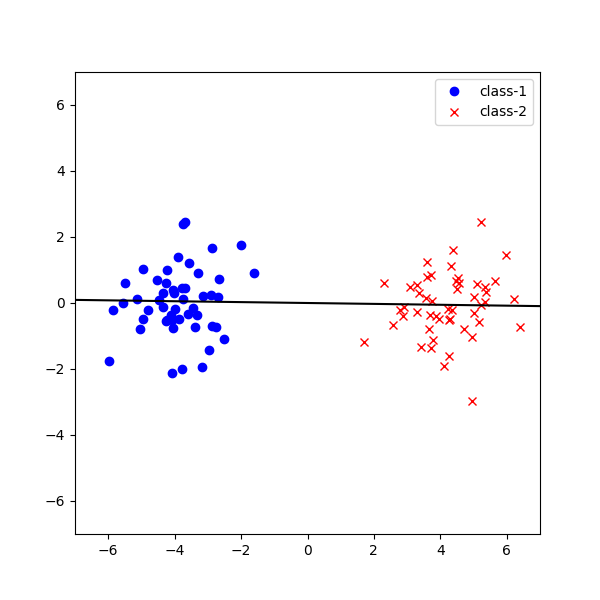
\includegraphics[clip, width=12cm]{../figures/assignment1_result_two_cluster}
    \caption{2クラスタのデータに対する結果}
    \label{fig:result_2cluster}
\end{figure}

\begin{figure}[H]
    \centering
    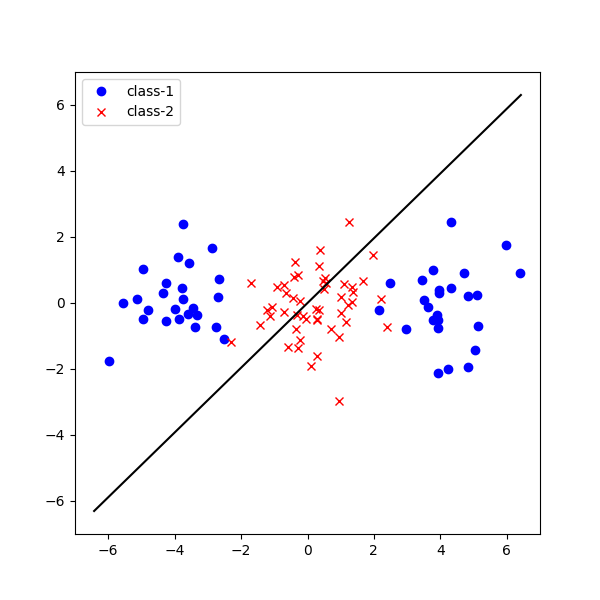
\includegraphics[clip, width=12cm]{../figures/assignment1_result_three_cluster}
    \caption{3クラスタのデータに対する結果}
    \label{fig:result_3cluster}
\end{figure}



\end{document}
